\section{Implementation}

\subsection{Setup}
\subsubsection{Hardware}
For development the Digilent Nexys-A7-100T development board has been used. It uses the Xilinx Artix-7 chip XC7A100T-1CSG324C. Reference manual for the development board can be found in \cite{digilent:nexys-a7-ref-manual}.
The board owns an ethernet PHY chip, model LAN8720A, manufacturer SMSC. This PHY is used to implement the physical layer of the OSI model. For pin connections to the FPGA consult the reference manual of the development board (\cite{digilent:nexys-a7-ref-manual}). For general information about the ethernet PHY, consult its datasheet (\cite{smsc:lan8720a}).

\subsubsection{Programming Environment}
For FPGA programming there are two programs to be used:
\begin{enumerate}
  \item \textbf{Xilinx Vivado (Current Version 2020.2):} This is the standard hardware development IDE to program Xilinx FPGAs. Hardware is described here in VHDL or Verilog. Also, custom and third-party modules can be used here.
  \item \textbf{Xilinx Vitis HLS (Current Version 2020.2):} This is the IDE to program custom modules in a higher level language (C, C++, or SystemC). It uses a guided workflow to program tested VHDL or Verilog modules out of the high level language. After successful development, the module can be exported and used within Xilinx Vivado.
\end{enumerate}

\subsubsection{Code}
The whole code is hosted on GitHub:
\begin{center}
    \url{https://github.com/pete-lennart/FPGA-Networking}.
\end{center}
In this project, C++ has been used as high level language and two modules have been created:
\begin{itemize}
  \item \textbf{Inbound packet handler:} This block reads incoming data from the RXD pins of the ethernet PHY and bundles the data to octets. Those octets are stored and checks are made, whether the checksums and addresses are correct and whether the packet is a UDP packet. Currently, only UDP packets are supported. If everything is correct, the UDP payload data is passed to the blocks output to be used by another block via an AXI-Stream port.
  \item \textbf{Outbound packet handler:} This blocks reads incoming data from an AXI-Stream port, wraps this data into a UDP packet (including IP and MAC packet) and passes it to the ethernet PHY pins TXD to be sent over ethernet.
\end{itemize}
Both handlers have been connected to each other, so that an echo server is established. In the future when other modules want to work with the incoming data, those modules have to be connected in between the inbound handler and the outbound handler.
A schematic of the connections can be seen in figure \ref{figure:schematic}.

\begin{sidewaysfigure}[h]
  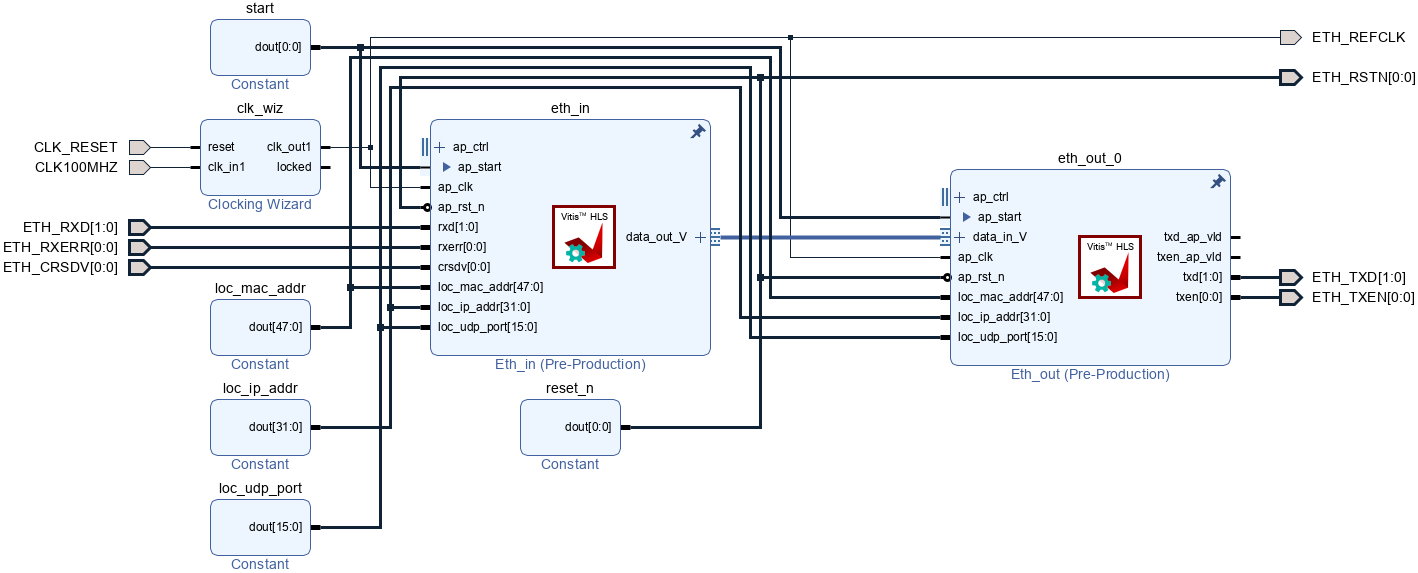
\includegraphics[width=\textwidth]{assets/schematic.png}
  \caption[Schematic of the UDP echo server implementation]{Schematic of the UDP echo server implementation. The left big block is the inbound data handler, the right big block is the outbound data handler. The outermost small grey nodes are the external pins, mostly pins of the ethernet PHY (ETH\_RXD, ETH\_RXERR, ETH\_CRSDV, ETH\_TXD, ETH\_TXEN, ETH\_RSTN, ETH\_REFCLK). Additionally, two ports for external clocks are used. Both handlers use predefined addresses for MAC, IP and UDP packets.}
  \label{figure:schematic}
\end{sidewaysfigure}

\subsection{Run}
\begin{enumerate}
  \item \textbf{Create ethernet handler:} Run \texttt{src/ethernet_handlers/build.tcl} of the github project within the Vitis HLS Command Line. In the end an IP directory is created, which contains both ethernet handlers in a form usable by Vivado.
  \item \textbf{Create the logic:} Create a new Vivado project and implement the schematic shown in figure \ref{figure:schematic}. Choose the addresses of the board as you need. UDP port and MAC address are not important, but IP address must be adjusted to match your connections subnet (first 16 bits of IP address). Otherwise the computer won't send any packets. Use both modules from step 1. To use them, create a new IP repository and add both modules to it. The constants \texttt{start} and \texttt{reset\_n} must be set to \texttt{1}.
  \item \textbf{Connection:} Connect the FPGA board with a computer via ethernet cable. The link status LED of the ethernet port should blink after connecting.
  \item \textbf{Set ARP entry:} ARP is a protocol mapping IP addresses to MAC addresses. In order to be able to send IP packets, both have to be known. ARP is not implemented on the board, therefore the entry has to be added manually. In windows this is done by executing \texttt{arp -s <IP\_ADDR> <MAC\_ADDR>} in a command line. For UNIX systems please consult the internet.
  \item \textbf{Program the board:} Run synthesis, implementation and bitstream generation of the echo server and program the board.
  \item \textbf{Send and receive packets:} Run the code udp client written in rust in the subdirectory \texttt{src/udp\_client} with the command \texttt{cargo run}. In order to run it, rust and cargo has to be installed. This program sends a byte and receives a byte, prints both to the console and measures the time between sending and receiving. IP addresses and UDP port must be adjusted for the local machine and the FPGA board.
\end{enumerate}
